%---------------------------------------------------------------------
%
%                          Cap�tulo 4
%
%---------------------------------------------------------------------

\chapter{Metodolog�as utilizadas}

\begin{FraseCelebre}
	\begin{Frase}
		" La fuerza no viene de la capacidad corporal, sino de la voluntad del alma". 
	\end{Frase}
	\begin{Fuente}
		Mahatma Gandhi
	\end{Fuente}
\end{FraseCelebre}


Introducci�n capitulo 4 COMPLETAR  y cambiar frase c�lebre
\\


%-------------------------------------------------------------------
\section{Reuniones}
%-------------------------------------------------------------------
\label{cap4:sec:Reuniones}

Para una buena organizaci�n, desde el principio el equipo de trabajo se ha reunido una vez a la semana para asignar las diferentes tareas, comentar el trabajo realizado y poner en com�n todos los conocimientos adquiridos por cada uno. A lo largo de la semana tambi�n hab�a reuniones a trav�s de Skype\footnote {\url{https://www.skype.com/es/}} para comentar y resolver las posibles dudas que podr�an surgir durante el proceso. \\

El equipo tambi�n se ha mantenido en contacto v�a email con los tutores comentando el estado del proyecto. A esto se a�adieron reuniones mensuales con ellos para realizar correcciones de la memoria, revisar el progreso, resolver dudas y comentar las tareas necesarias para las siguientes fases.\\

De esta forma, los integrantes del equipo y los tutores han estado informados constantemente del progreso del trabajo, se ha podido hacer un reparto claro de tareas y se han podido establecer tiempos de entregas realistas y factibles.\\

%-------------------------------------------------------------------
\section{Trello}
%-------------------------------------------------------------------
\label{cap4:sec:Trello}

A lo largo de todo el proyecto se ha utilizado la herramienta Trello\footnote {\url{https://trello.com/}} para el reparto claro y equitativo de tareas entre los componentes del equipo de trabajo. Trello consiste en un conjunto de tableros, a los cuales se les pueden a�adir una serie de tareas con diferentes estados. Esto podemos observarlo en la Figura X, donde se muestra un ejemplo de tablero utilizado en el desarrollo del proyecto. Esta herramienta permite ver de manera sencilla el estado del proyecto, facilitando as� la organizaci�n de las tareas a realizar. En el desarrollo de ``Text2LSE'' se han utilizado tres tableros distintos:

\begin{itemize}
	
	\item \textbf{Investigaci�n:} Incluye las tareas relacionadas con toda la investigaci�n referente al proyecto, como por ejemplo LSE, Python, PLN, etc.
	
	\item \textbf{Desarrollo:} Este tablero contiene las distintas tareas de desarrollo de c�digo, tanto de la aplicaci�n web como de la API.
	
	\item \textbf{Memoria:} En este tablero se encuentran las distintas tareas relacionadas con el desarrollo y correcci�n de los apartados de la memoria.
	
\end{itemize}

Para una mayor organizaci�n, cada tablero se ha estructurado en tres estados:

\begin{itemize}
	
	\item \textbf{Lista de Tareas:} Lista de tareas asignadas a un miembro del equipo en concreto que todav�a est�n sin empezar.
	
	\item \textbf{En proceso:} Tareas que el propietario de la tarjeta tiene en proceso de desarrollo. 
	
	\item \textbf{Hecho:} Tareas completadas y subidas al repositorio de GitHub.
	
\end{itemize}

Cada miembro del equipo ha sido el encargado de actualizar en tiempo real el estado de las tarjetas que ten�a asignadas. De esta manera se ha conseguido tener una buena organizaci�n con respecto a las tareas a realizar.

%\begin{figure}[]
%	\centering
%	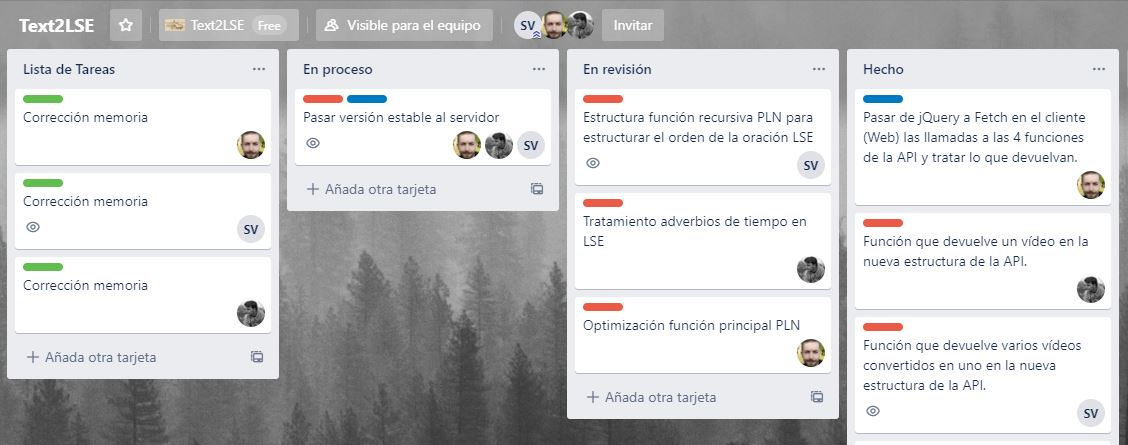
\includegraphics[width=1\textwidth]{Imagenes/Fuentes/Metodologias/trello.png}
%	\caption{Tablero \textit{``Memoria''} utilizado en el proyecto.  }
%	\label {fig: imgTrello}
%\end{figure}
% ~\ref {fig: imgTrello} -> elegir imagen de tablero









